\subsection{Великая игра}
\textit{Этот фрагмент проговариватся словами, на фоне видеозапись со мной и моей речью, где на заднем плане Зимний дворец, Кадр 1}


Одним из самых острых вопросов располагался в средней Азии.

\textit{Вывожу карту}
\newline 
{\centering 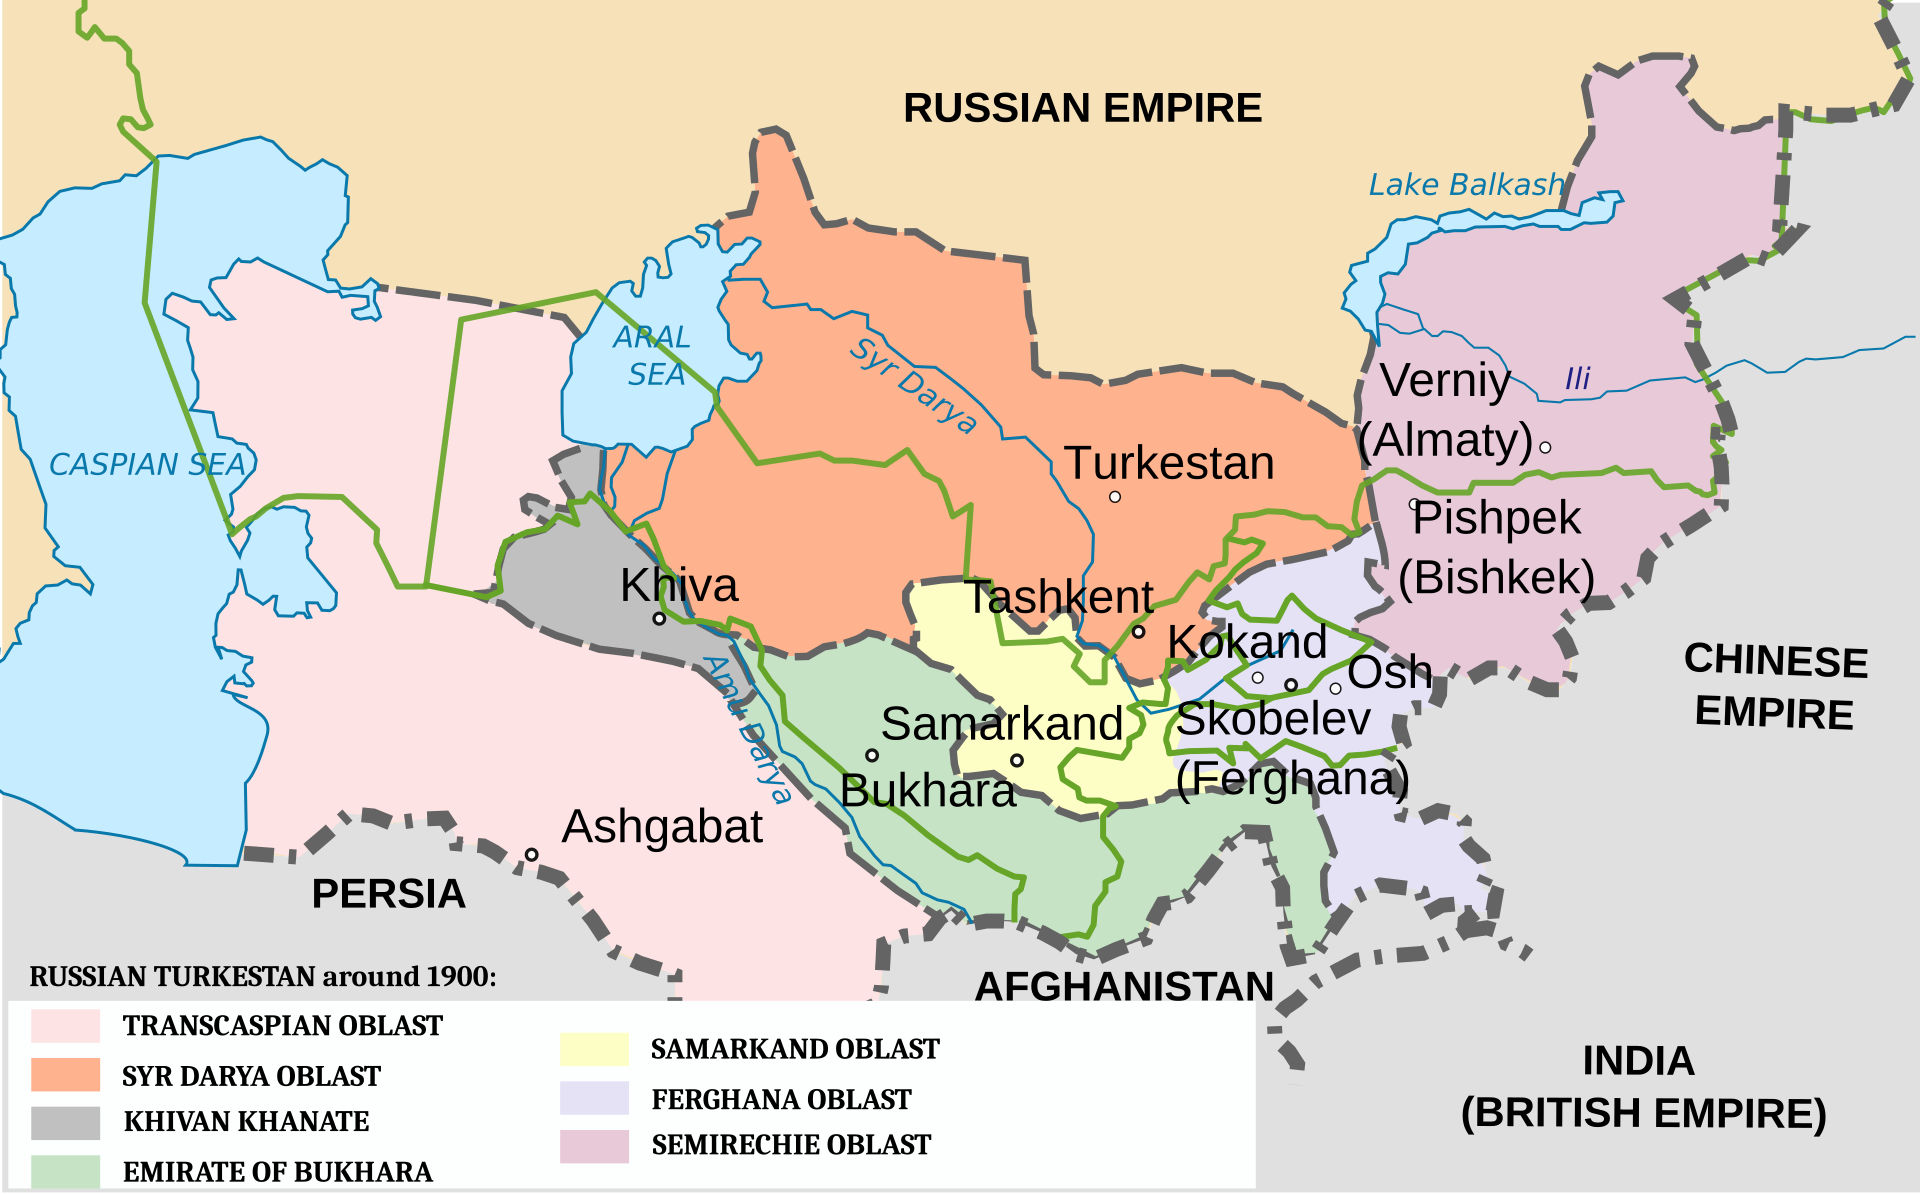
\includegraphics[width=\textwidth]{images/Turkestan_1900-en.png}}

На протяжении всего XIX века Россия активно расширяла свою зону влияния в этом регионе. За этот век удалось подчинить себе территории всей центральной Азии и подойти к границам Персии, Афганистана и Индии

\textit{Возвращаюсь к Кадру 1}

Что весьма озаботило Британское правительства, т.к. для их "Жемчужины империи" - Индии появилась явная угроза вмешательства в функционирование государства. Прямое вторжение с целью захвата было маловероятно, но Британцев беспокоила сама возможность оказания влияния на эту колонию, например, через организацию переворотов. Или через необходимость стягивания военной силы в Индии т.к. Россия могла послать туда армию, чтобы растянуть силы оппонента, например, пока Россия пытается взять Константинополь, чтобы уже наконец получить свободный выход в Средиземноморье. Чего Британская империя крайне боялась, ведь это значило бы появление нового сильного игрока в мировом океане, который Британия считала свой зоной влияния. 


\textit{Вывожу карту}
{\centering 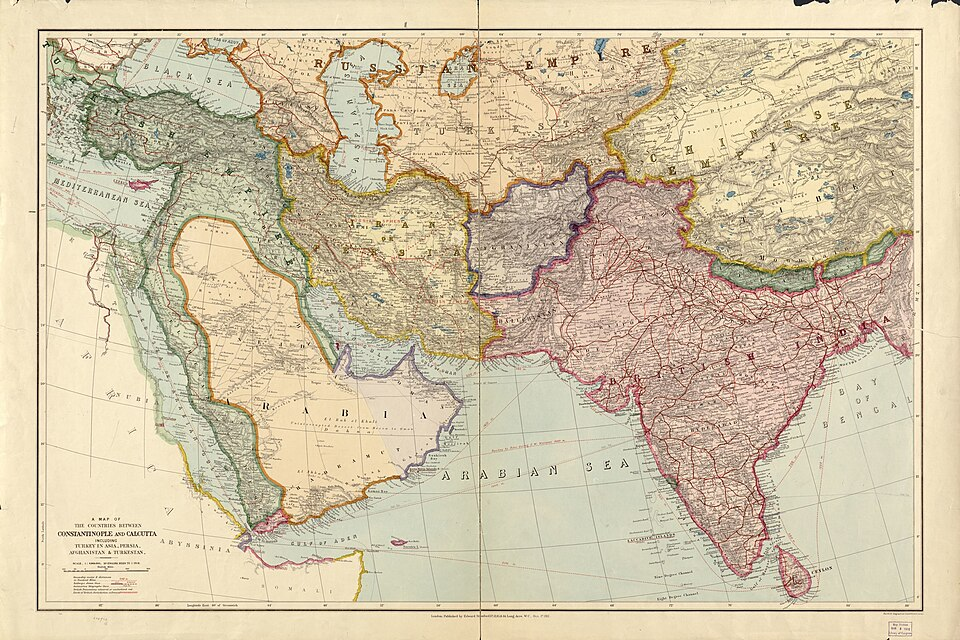
\includegraphics[height=0.3\textheight]{images/Политическая_карта_Азии_начало_XX_века.jpg}}


Выход в мировой океан Россия могла получить и взяв Персию под свой полный контроль, что также крайне не устраивало Лондон, ведь это означало бы, что поток товаров из Индии находится под угрозой. 

\textit{Возвращаюсь к Кадру 1}

Из-за чего Британия мешала продвижению России дальше в регион. Этот региональный конфликт смог окончательно решиться в 1907 году, подписанием Англо-Русской конвенции.